\documentclass[../main/main.tex]{subfiles}

\newdate{date}{09}{04}{2020}

\begin{document}

\section{Lecture 10}
 \displaydate{date}. Compiled:  \today. Alice.
 

\subsubsection{Slide 157}

\begin{figure}[h!]
\centering
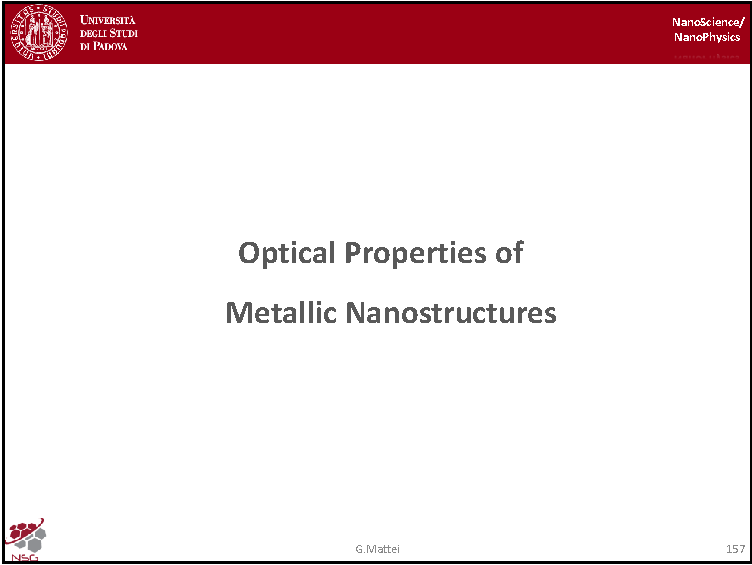
\includegraphics[page=1,width=0.9\textwidth]{../lessons/pdf_file/10_lesson.pdf}
\end{figure}

We want to describe the basic physics which describe when light interacts with matter in metallic form at the nanoscale. Plasmonic is a term used to describe interaction between photons and free electrons.

We will see how to obtain controlled properties due to controlled synthesis we have seen into the previous lectures.

\newpage

\subsubsection{Slide 158}

\begin{figure}[h!]
\centering
\includegraphics[page=2,width=0.9\textwidth]{../lessons/pdf_file/10_lesson.pdf}
\end{figure}

Some beautiful example of what apparently has no relation with plasmonic but which has a very profond link with optical properties at the nanoscale.

The first figure is a glass cup decorated with gold (roman did it in the four century).
It has peculiar optical properties indeed if you see this cup illuminated by Indium lightnening, that is if you see the cup illuminated in reflection (the cup will reflect the ambient light), the color apparently is green like in this picture.

But if you put mole blump inside the cup and you look the color in transmission the color appears red as in the second picture.
It is a quite strange phenomenum, the cup is not painted with some painting which produce the color but the color is the biproduct of the interaction between light and the structure.

Of course we now the composition of the glass of this cup, which is an amorfous glass and it is a mixture of different oxide.
In particular, the composition of the Lycurgus cup is not so different from the composition of the modern so called soda-lime glasses.

At that time now one was able to explain why the optical property of the cup changed with the change of the illumination in the system. People in the year develop a receip in how to convey the optical properties in terms of controlling the color of a glass.
A close solution of the problem was given in the early years of the 20 century by Gustav Mee (we will see his theory based on electrodynamics as able to quantitavely prdict this behaviour).


The composition of the Lycurgus cup glass was an allow of gold ans silver with average size of 70nm.
Why does the intrusion of the alloy of golden and silver are responsible for the change of color? The soda-lime glass by itself is not able to produce th is kind of phenomena, it is just transparent like in the windows.

\newpage

\begin{figure}[h!]
\centering
\includegraphics[page=3,width=0.9\textwidth]{../lessons/pdf_file/10_lesson.pdf}
\end{figure}


\begin{figure}[h!]
\centering
\includegraphics[page=4,width=0.9\textwidth]{../lessons/pdf_file/10_lesson.pdf}
\end{figure}

\subsubsection{Slide “La Sainte-Chapelle”}
The window shows these beautiful colors (blu, red) and also in this case the color is not given by some paintings but it is given in something that is inside the glass.

\subsubsection{Slide “Chartres Cathedral”}
Those are other examples.


\newpage

\subsubsection{Slide 161}

\begin{figure}[h!]
\centering
\includegraphics[page=5,width=0.9\textwidth]{../lessons/pdf_file/10_lesson.pdf}
\end{figure}

Another kind of nanotechnology not based on glass is the “Lustres in Gubbio and Deruta”. The technology for producing this beautiful decoration of the dishes is still based on nanotechnology, because the colors is not given by pigments but if you are able to look at the microscopic structures of those dished, the decoration which is called Lusters, you can see the nanostructure in figure 2. The image is obtained by electron microscopy and you can see nanoparticles with different compositions: copper and silver nanoparticles (not an alloy of that but just separated). However, you can see that the size is very very small with respect to the 16th century technology.

People could understand that the color was given by different compositions of the copper and silver contained in the decoration. The reicipe for the Lustre is reported here.
The recipe is very similar to the modern recipe to obtain very similar nanoparticles.

In this case the matrix is a sort of silicate glass and the dishes before the position of the luster is painted by zinco oxide which is a sort of total white background so that the optical properties of those parts is controlled by the reflection. Light is able to pass trough the transparent luster, it is back reflected by the zinco oxide white layer so that we can see the transmitted color through the decoration.

\newpage

\subsubsection{Slide 162}

\begin{figure}[h!]
\centering
\includegraphics[page=6,width=0.9\textwidth]{../lessons/pdf_file/10_lesson.pdf}
\end{figure}

If we quantitavely want to measure the optical properties of the luster we can see for istance these tiny fragment of the dishes.

If we measure the optical density that is the intensity at that specific frequency (or wave length) if we look at the visible range, you see that the  gold color has a distribution of intensity is not homogeneous but it shows the main peak around the extreme range toward the ultraviolent range and another tiny showed around 600nm.

If we look at the reddish color in another piece we measure spectrally the intensity of light reflected by the dishes and in this case we have a more homogeneous distribution with two tiny peaks and a tiny shoulder.

You can clearly understand that the luster color is linked to its optical properties. According to the spectral distribution of intensity, you can obtain different colors. This is the RGB technique (by changing the relative ratio between these colors you can obtain the color that you want), so the concept is exactly similar but done in analogic way and not selfware.

\newpage

\subsubsection{Slide 163}

\begin{figure}[h!]
\centering
\includegraphics[page=7,width=0.9\textwidth]{../lessons/pdf_file/10_lesson.pdf}
\end{figure}

We have a silica glass implanted in our lab just to show you that we can produce something which is quite similar to the Lycurgus cup and that we can anderstand what is going on.

The red bans is the place where ion beams was rustered (with respect to the white band, where the sample was not implanted due to a mask). We remind that ion implantation is very flexible in the sense that it is able to produce micropatterning in the substrate that you want to nanofabricate.
However, what is important now for us is that we have a glass implanted that is on top of a white screen. Basically we see a light that, as in the Lusters, is entering in the system and that is back reflected from the substrate (so we see in trasmittance what is going on).

If we look at the microscopic structure at electron microscope  we have those beautiful nanoparticles. In this particular case we produce the sample by sequential ion implantation:
\begin{enumerate}
\item we implanted first gold;
\item then we implanted silver at the very same fluence with a different energy in order to overlap the two spatial concentrations (so that promoting alloying);
\item then we annealed thermally in air at 800° for 1 hour.
\end{enumerate}
From electron diffraction (of the very same sample) we can confirm the structure is the FCC structures of both silver and gold in an alloy. In the TEM we can measure directly the composition of the nanoclusters trhough the x-rays emitted as biproduct of the interaction between the incoming electrons and atoms in our system.

If we do an analysis of the structure we see that the histogram of size produce an average size of size produce an average size of 9nm (we have a sample very similar to the nanoclusters within the Lycurgus cup). The composition in this case is slightly enrich in gold.

It is instructive what is going on in the system and try to understand the optical properties in a controlled way.
We notice that in the histrogram we have a bimodal size distribution which you could already recognize as a fingerprint of the onset of Ostwald ripening in the system. You see that indeed the clusters are quite large and well defined so there is no supersaturation remained.


\newpage

\subsubsection{Slide 164}

\begin{figure}[h!]
\centering
\includegraphics[page=8,width=0.9\textwidth]{../lessons/pdf_file/10_lesson.pdf}
\end{figure}

In general we have seen that by using ion implantation we are able to produce nicely nanocomposits (that is a composit material, or metal material).
We have a dielectric matrix (a glass) containing metall nanoparticles.

\newpage

\subsubsection{Slide 165}

\begin{figure}[h!]
\centering
\includegraphics[page=9,width=0.9\textwidth]{../lessons/pdf_file/10_lesson.pdf}
\end{figure}

If we look at this example, we have the gold nanoparticles obtained by ion implantation of gold (we remember the gaussian like profile of the implantation species and all the properties we can control by controlling the energy, as the projected range, the straggling, or the maximum concentration by controlling the fluence).

\newpage

\subsubsection{Slide 166}

\begin{figure}[h!]
\centering
\includegraphics[page=10,width=0.9\textwidth]{../lessons/pdf_file/10_lesson.pdf}
\end{figure}

Ion implantation can do not only single species implantation but it is aquite clever technique for nanofabricating metallic nanostrutures. You can play with the size by controlling the concentration that you deposited in the system. You can with the structures, for instance you can obtain in a controlled way different crystallografic structures for the very same system (for instance Cobalnt normal has a structure hcp, but at the nanoscale the fcc is esoenergetic). You can do more, if you do sequential ion implantation (that is you implant a species, then another species and so on, hence you can obtain multicomponent system) you can play also with the composition, that is you can obtained alloyed of multicomponents nanoparticles like in this example in which we have gold-copper alloyed nanoparticles (mixture of the two).
It is very important, because normally the best performance are obtained no by single element systems, but by mixing elements.
In particular, you can obtain an alloying of elements which are not mixible in the bulk.

\newpage

\subsubsection{Slide 167}

\begin{figure}[h!]
\centering
\includegraphics[page=11,width=0.9\textwidth]{../lessons/pdf_file/10_lesson.pdf}
\end{figure}

here we report the golden-silver binary phase diagram, which is very simple because the two elements shares the very same cristallographic structure (fcc) and the lattice parameter is remarkably similar. Moreover the two elements are noble metals, so they share structures, electronic properties, so they are mixible at any composition.

A solid solution means that you have a well defined structure (the soldi crystalline), but the occupancy of the size in this fcc cell (you may remember you have 4 different atoms per unit cell) is stocastical (you have a fraction of occupancy which is triggered by the local composition), but locally you have an order structure. So it is structurally order and chemically disordered.

\newpage

\subsubsection{Slide 168}

\begin{figure}[h!]
\centering
\includegraphics[page=12,width=0.9\textwidth]{../lessons/pdf_file/10_lesson.pdf}
\end{figure}

The situation is quite similar if you look at gold-copper binary phase diagram. At lower temperature in this case, something new appear. We have three chemically ordered phases.  That is the four atoms in the fcc structures are well controlled. So those are also chemically ordered phases.
You can see that as before you can obtain an alloying at any composition by controlling temperature.

Of course you can obtain a quencing from the liquid phase, so you can trap the structure in a metastable state. That is if you quench from high temperature and you reduce rapidly the temperature, you can trap the system in a metastable state, but when you anneale under thermodynamic equilibrium the structure will relaxe in the most stable structure from a thermodynamic point of view.

\newpage

\subsubsection{Slide 169}

\begin{figure}[h!]
\centering
\includegraphics[page=13,width=0.9\textwidth]{../lessons/pdf_file/10_lesson.pdf}
\end{figure}

The situation is different in the case of silver and copper, because at room temperature there is no change to obtain an alloying between the two metals. From the liquid if you go down you have decomposition of the two subsystems (basically you end up in decomposition of copper separated by silver). You can obtain a metastable alloy if you quench from the liquid phase, but as mentioned in this case is really hard to stabilize the structure and any increase in the temperature will tends to decompose the system.

For that reason the Lusters decoration we have silver and copper as separated phases and not as an alloyed in contrary of the Lycurgus cup in which we have an alloy of golden-silver.

\newpage

\subsubsection{Slide 170}

\begin{figure}[h!]
\centering
\includegraphics[page=14,width=0.9\textwidth]{../lessons/pdf_file/10_lesson.pdf}
\end{figure}

The situation is even more complicated if you try to mix a noble metal as gold with a transition metal as iron. Magnetic properties are quite interesting application for what is called magnetoplasmonics, that is the ability to combine magnetic and optical properties at the nanoscale with metallic nanoparticles.

As you can see we have a lot of different phases, but when we go down at any composition of iron normally at room temperature you are not able to obtained an alloyed system. But from any composition you arrive you will be driven toward separated phases, because the two elements are not mixible at room temperature in the bulk phases.

But again we are able for instance with ion implantation to obtain well controlled composition of gold-iron nanoparticles and we measure there magneto optical proeprties.

So the basic rules that you can obtain is that those are bulk binary phase diagrams, but at the nanoscale rules are broken basically by the surface and by the chance to stabilize in metastable phase if you work out of the thermodynamic equilibrium.

\newpage

\subsubsection{Slide 171}

\begin{figure}[h!]
\centering
\includegraphics[page=15,width=0.9\textwidth]{../lessons/pdf_file/10_lesson.pdf}
\end{figure}

If we do sequential ion implantation of gold and copper, we can use the very same fluence (same amount of elements in the system, silica in this case).

We can simulate the expected concentration profiles (fig.1) by triggering the energy. If you can can match the projected range you increase the probability of interaction between the two subsystem and promote alloying.

In principle, you are not sure that you will obtain an alloying instead of separating phase. One rule could be the mixibility in the bulk, but in general if you sequential implant two elements \textbf{A} and \textbf{B} in a very same system you could end up into three different morphologies:
\begin{itemize}
\item (fig.2) the first is that the two subsystem do not mix, basically so you will end up into two separated subsystems, one of phase A and one of phase B (as in the silver-copper system in the Lustre decoration);
\item (fig.3) you can obtain an alloy that is a favorable situation, because you can control the properties not just by addition, but just changin the electronic structure of your system;
\item (fig.4) or you can end up in a different situation in which you have separated precipitation of the two phases but in a coordinate topology. You end up in what is called \textbf{core-shell} system, in which you can have a core of species A decorated by a shell of species B. It is can be also very useful for controlling and modulating the global properties of the material that you nanofabricated with this technique.
\end{itemize}
How are we able to obtain one of this possibilities? We have to develop suitable nanofabrication recipes to obtain one of the three structures.

\newpage

\subsubsection{Slide 172}

\begin{figure}[h!]
\centering
\includegraphics[page=16,width=0.9\textwidth]{../lessons/pdf_file/10_lesson.pdf}
\end{figure}

Ion implantation:
\begin{itemize}
\item If we want to promote the interaction between the two species, when we work with ion implantation we can play with the energy, fluence to maximize the spatial overlapping of the two concentration profiles.
You can have multiple energy implantation to promote a better uniformity in concentration.

\item Of course, you need to take into account the miscibility of the implanted elements that is the variation of the hentalpy of mixing when you try to combine the two subsystems. So you want to study what is called nano-alloying, that is alloying at the nanoscale, which as mentioned will follow rules which are not as the one in the bulk.

\item You can also play with the chemical interaction with the matrix. If you implant gold and copper, copper will be more reactive with the oxigen in the matrix with respect to gold. The order of implantation will have tremendous impact. If you implant first copper probably in a copper-oxide system, but if you implant first gold and then copper, the already formed gold nuclei will tends to stabilize the metallic alloying.

\item You can have radiation-induced defects. During ion implantation you produce a lot of defects as we have seen in the simulations and those can promote an accelerated diffusion, because you may remember that diffusing species will move faster around defects. SO the energy barrier is lowered by the disordered structure.
\end{itemize}

Of course you can play also with the post-implantation annealing or irradiation (as we have seen for the nanoplanets case).

\begin{itemize}
\item So if you play with the athmosphere of annealing you can exploit different chemical interaction with the species in the athmosphere of annealing. For instance if you have oxigen, you can play with the interaction between the two elements with the oxigen in the system.

\item Or you can play with the temperature to control the radiation induced defects and to control therefore the diffusivity of your system.

\end{itemize}

\newpage

\subsubsection{Slide 173}

\begin{figure}[h!]
\centering
\includegraphics[page=17,width=0.9\textwidth]{../lessons/pdf_file/10_lesson.pdf}
\end{figure}

Let us look at the optical properties from an experimental point of view. Let us see first how the controlled syinthesis that we have seen with ion implantation can help us in understanding the evolution of the optical properties.
We start with optical properties in the linear regime, that is the usual regime in which we will work. In the end of the course we will briefly touch non linear optical properties, but it is more complicated to understand.

\newpage

\subsubsection{Slide 174}

\begin{figure}[h!]
\centering
\includegraphics[page=18,width=0.9\textwidth]{../lessons/pdf_file/10_lesson.pdf}
\end{figure}

Let us see how the optical properties of gold nanoparticles obtained by ion implantation in silica can be measured and described.

You may remember that we were able to produce nicely controlled gold nanoparticles in silica implanted with that energy and fluence. We controlled as a function of the annealing time the average radius of the system. So we have a perfect playground for testing the evolution of the optical properties as a function of the size in our system, because we know exactly what is going on in terms of average nanoparticles size.

The typical experiment that we do (we will see it in experimental activity) is the so called \textbf{Lambert beer experiment}. You have your system with the set of nanoparticle.

For instance we can have a solid matrix with a liquid solition of nanoparticles (whaterver is our system). Let us suppose the thickness is \( z \) and you shine light (can be monocromatic or in general is monocromatized but scanned in frequency, so that you have a spectral representation of the interaction between the incoming beam) from one side of your sample to the other side. Indeed, you will measure the light emerging in the very same direction of the incoming light, but after the interaction of the system. So you will end up in intensity which is a function of the thickness of your system and of \( \lambda  \).

The spectral dependency of the intensity is related by the exponential exctintion of light due to the interaction either in form of absocron or scattering by the structure and those properties are summarized by this \( \gamma   \) function which has a spectral dependence (is a function of wave length).

You can define the trasmition function which is the ratio between the emerging intensity with respect to the incoming intensity. Or you can define the absorbance.
Unfortunatly for historical reasone people use the ten logarithm instead of the nantural logarithm. The absorbance since it is directly proportional to the spectral interesting quantity (\( \gamma   \)).
The \( \gamma   \) will be
the subject of our investigation in the following. Of course \( z \) is just a multiplicative constant in our system.

So by scanning the wavelength we can have a spectral representation of the interaction between a plane wave (which represents the incoming beam) and our system (in this case gold nanoparticle silica).

Normally the scan is done from the near ultraviolet range (200nm) up to the visible and near infrared (\( 2-2.5 \mu m \)). You can have very accurative information on the spectral behaviour of your system in the UV, VISIBLE and near INFRARED range.

Let us see what is going in the system.

\newpage

\subsubsection{Slide 175}

\begin{figure}[h!]
\centering
\includegraphics[page=19,width=0.9\textwidth]{../lessons/pdf_file/10_lesson.pdf}
\end{figure}

Those are the the intensity of your system and you have this evolution as in fig.2.
Basically I just restricted the spectral range in the visible range.
As a function of the annealing time we can see that optical properties changes (we obtain different spectra with different annealing time). The optical density is nothing but the absorbance.

We see that the spectron as a function of the wavelength is not uniform, but already in the as-implanted sample exibits a peak, which is called the \textbf{surface plasom resonance} (SPR). That is the resonance (the peak) is triggered by the plasmonic properties triggered by the surface (finite size of the metallic nanoparticles, as we will understand).

By increasing the annealing time, the resonant bands starts to increase as well and the full width half maximum will reduce.
The position of the resonant is almost constant, but the intensity is dramatically different as a function of the size.
This means that if we can control the size, we can control the optical properties.

To better understand why this resonant is not symmetric takes more physical understanding, but for the moment let us stay on the experimental side.
So we phenomenologically see that controlling the size is a way to control the optical properties.

\newpage

\subsubsection{Slide 176}

\begin{figure}[h!]
\centering
\includegraphics[page=20,width=0.9\textwidth]{../lessons/pdf_file/10_lesson.pdf}
\end{figure}

If we look at the optical properties not of a single component system but of a binary alloyed like in the case of golden-silver alloy (obtained by sequential ion implantation in silica and subsequent thermal annealing, as we have seen).

\newpage

\subsubsection{Slide 177}

\begin{figure}[h!]
\centering
\includegraphics[page=21,width=0.9\textwidth]{../lessons/pdf_file/10_lesson.pdf}
\end{figure}

The picture which emerges is the one in figure. Those are the spectra obtained in the very same geometry as described before for the different samples we have considered.

So for better understand what is going on on our system, we compared the optical properties of pure separated system with respect of the alloyed system and atdifferent stages of post-implantation annealing.

Let us see how the samples are produced:
\begin{itemize}
\item For the green one. We implanted first gold and then silver. The label is \( Au3Ag3 \) means that we used the very same fluence (that is \( 3 \times 10^{16} \, ions/cm^2\)) and we tuned the energy of the two ions in order to have the maximum overlap in depth (so that they have exactly the same projected range) in a way to maximize the chance to have an alloying. Indeed, we have an alloying.

\item For the red term \( Au3Ag3H \), the \( H \) means that we are describing annealing athmosphere. In particular, we used an annealing at \( 800° \) for 1 hour in reducing athmosphere of argon containing \( 4\% \) of hydrogen, just to promote reduction and to use more or less the very same recipe of the Lycurgus cup.

\item For the blue term \( Au3Ag3A \), the \( A \) means that we performed an annealing at the very same temperature for 1 hour but in oxidizing athmosphere.

\item The gray and pink samples are just the monoelemental samples (just gold or silver) at the very same fluence and we annealed them in the oxidizing athmosphere.
\end{itemize}
If we look at the position of the resonances we note the dramatically different intensity of the resonance in the case of pure silver with respect to pure gold.
This is because the melting temperature of gold is larger than the melting temperature of silver. For silver \( 800° \) is very high temperature, so the diffusivity is quite large. But also the diffusion coefficient of silver is much larger in silica with respect to that of gold, even if we are exploiting the correlated diffusion concept already discussed.

If we look at the tiny resonant of pure gold with respect to pure silver, the spectral position of these resonance is respectively at \( 407nm \) and \( 530nm \).
So the first observation is that apart from the intensity, the spectral position of the resonance is a function of the material. Hence, changing the composition we can change the optical properties.
So the size matters, but also the composition for determining the optical proeprties!

We would like to have a modulated system in which we can control continuously the position of these resonance (from the one of pure silver toward the one of pure gold). The easiest way from a conceptual point of view is to try to have an alloying, because if you could have a separated system you will end up just in a linear combination of the two, there is no chance to have the resonance between them but just a combination of two resonances.
So if you want to have a resonance in between, you need to obtain an alloying.

\begin{itemize}
\item If we look at the as-implanted sample (the sample just after the implantaion (first gold and then silver)), the position of the resonance is around \( 501nm \), so it is in between with respect to the pure elements, but if we consider that we are implanting in the very same amount of the two elements we would expect to have something exactly in between. Why is not exactly in between? The explanation of this is that probably we have still modifying the composition of the already formed gold nanoparticles. You may remember that even after ion implantation without thermal treatment in the as-implanted sample of gold we still have already formed gold nanoparticles. So they are stable nanoparticles so the additional arrival of silver ions, can be stabilized even on the already formed nanoparticles. But of course, an amount of silver ions are not entering directly after the implantation within the already formed gold nanoparticles.
So we can expect that we have part of the silver ions still in the matrix nad just a tiny fraction of them entering the alloying. It is as if the alloying was very rich in gold, which is nice because this means that we can move slightly the resonance toward the one of the silver system.

\item If we do the thermal annealing in reducing reducing or oxidizing atmosphere what we obtain is exactly what we expected. Because we have two resonances which are exactly in between (\( 435nm \)) but the intensity of the sample annealed in air is slightly larger with respect to the sample annealed in reduced athmosphere. This is not surprising, we may remember the effect of annealing atmosphere in the diffusivity of the species inside the matrix. The correlated diffusion of gold is a sort of very efficient boost to promote diffusion. So that already with reducing atmosphere we brought all the disperses silver atoms in the matrix into the nanoparticles, but the average size is slow. When we add the oxigen in the atmosphere (axidizing atmosphere) all the nucleation is faster and all the growth is faster and we obtain larger nanoparticle, hence we have an increasing in intensity.
\end{itemize}
The picture that emerges here is that if we can control the composition of the alloying, we can control the position of the optical resonance and if we can control the optical resonance in a very naif picture we can control the color of the system.
With this control you can control the interaction of your system with suitable optical phenomenum occurring at that specific wavelength and at that specific range.
For instance if you want to promote absorbtion of you structure at a specific wavelength, you would better use alloying system with respect to pure system.

But for the moment let us stay on this remarkable result, that is controlling the composition you can control the position of the resonance. It is a sort of linear combination in terms of the two positions and not just a linear combination in terms of the  intensities (otherwise you would have two resonances with different proportions!). This result remind the \textbf{Vegard's law} for the lattice parameters: when you have an alloy and you start from two similar unit cells (like in this case, in which you have two fcc cells) and the lattice parameter of the resulting alloying will be a linear combination of the lattice paramaters of the two original structures:
\begin{equation*}
  a_{AB} = x a_A + (1-x)a_B
\end{equation*}
this is the linear interpolation between the two orignal lattice parameters when you are forming an alloying between species \( A \) and \( B \) with this stechiometry: \( A_xB_{a-x} \). So the stechiometry can be used as a sort of weuight for triggering the structural properties of the alloying.
In the case of optical density we obtain a similar result: we are almost in between like in the Vegard's law for the structural evolution of the alloying.

\newpage

\subsubsection{Slide 178}

\begin{figure}[h!]
\centering
\includegraphics[page=22,width=0.9\textwidth]{../lessons/pdf_file/10_lesson.pdf}
\end{figure}

Now we look at the structure of our alloying as we have already seen. By TEM (fig.1 and 2) we can obtain quite larger structures whose composition can be measured by x-ray measurements within the electron microscope or to confirm from more fundamentl point of view the alloying we used technique which is called \textbf{EXAFS} (extended x-ray absorbition fine structures) based on syncrotron radiation that is a very coherent x-ray radiation which can be made resonant to the absorbtion edges of the two elements. So that you can investigate the environment around a single atom in the structure (in a statistic way of course) and then you can build a sort of correlation function of the atoms which are around the atoms you are probing (=sondare) and so you can have direct access to the composition of nearest neighbours with respect to that atoms and the number of nearest neighbours in your system. With this technique we do not want to enter in detail but we were able to confirm even better that our system was composed by a controlled alloying of gold and silver (fig.3).

At this point we need at theory which will help us to transform those phenomenological result into something that we can unrestand from a very fundamental point of view. This will be the subject of the next lessons.

\clearpage


\end{document}
